\documentclass{article}

\usepackage{graphicx}
\usepackage{tikz}
\usepackage{tikzsymbols}
\usetikzlibrary{calc,patterns,shapes.geometric}
\pagestyle{empty}
\usepackage[margin=0pt]{geometry}
\geometry{papersize={14in,12in}}

\def\centerarc[#1](#2)(#3:#4:#5){\draw[#1] ($(#2)+({#5*cos(#3)},{#5*sin(#3)})$) arc (#3:#4:#5);}

\begin{document}
	\begin{figure}
		\centering
		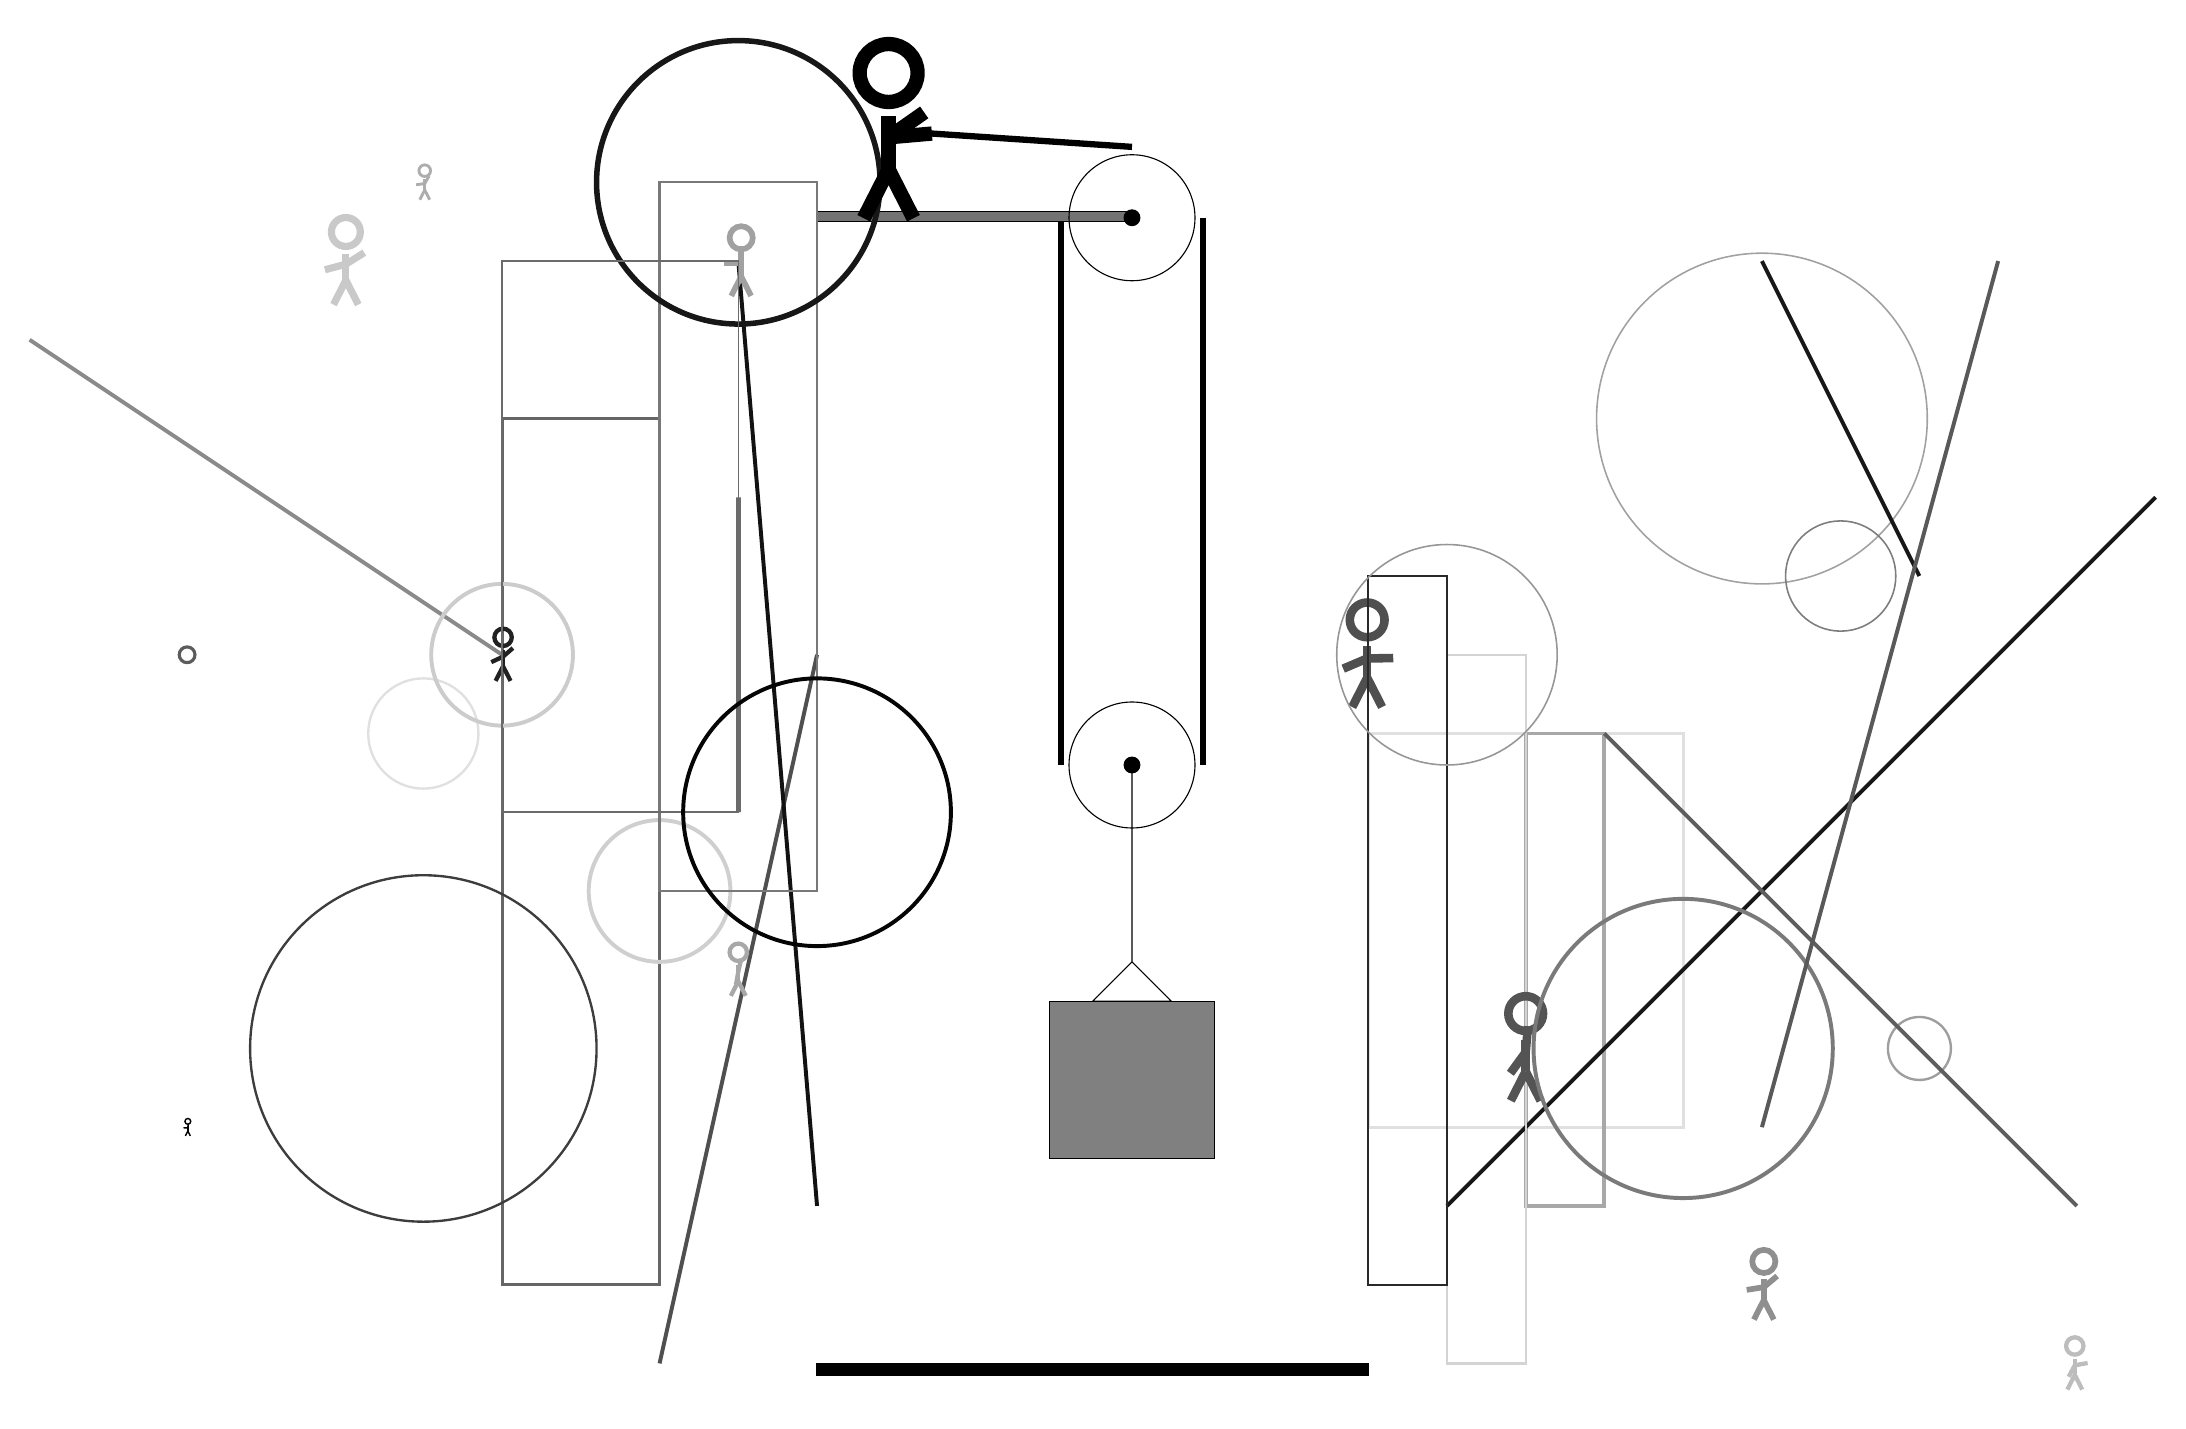
\begin{tikzpicture}
			%%%%% START %%%%%
			
			\draw[fill=black!55] (-2, 11.5) rectangle (2, 11.625);
			
			\draw (2, 4.6) circle (0.8);
			\draw[fill=black] (2, 4.6) circle (0.1);
			
			\draw (2, 11.55) circle (0.8);
			\draw[fill=black] (2, 11.55) circle (0.1);
			
			\draw (2, 4.6) -- (2, 2.1) -- (1.5, 1.6) -- (2.5, 1.6) -- (2, 2.1);
			\draw[fill=black!50] (0.95, 1.6) rectangle (3.05, -0.4);
			
			\draw[line width=0.8mm] (1.1, 11.5) -- (1.1, 4.6);
			\centerarc[line width=0.8mm](2, 4.6)(180:360:0.9);
			\draw[line width=0.8mm](2.9, 4.6) -- (2.9, 11.55);
			\centerarc[line width=0.8mm](2, 11.55)(0:90:0.9);
			\draw[line width=0.8mm](2, 12.45) -- (-1, 12.65);
			
			\draw[line width=0.4mm, color=black!12] (5, 5) rectangle (9, 0);
			
			\draw [line width=0.2mm, color=black!37](10, 9) circle (2.1);
			\draw[line width=0.6mm, color=black!58] (-3, 4) rectangle (-3, 8);
			\node[line width=0.5mm, color=black!44] at (10, -2) {\Strichmaxerl[4][9][40]};
			\draw [line width=0.3mm, color=black!12](-7, 5) circle (0.7);
			\draw[line width=0.4mm, color=black!60] (-4, -2) rectangle (-6, 9);
			\draw[line width=0.5mm, color=black!46](-6, 6) -- (-12, 10);
			\node[line width=0.3mm, color=black!32] at (-7, 12) {\Strichmaxerl[2][8][60]};
			\node[line width=0.4mm, color=black!99] at (-10, 0) {\Strichmaxerl[1][1][84]};
			\draw [line width=0.2mm, color=black!51](11, 7) circle (0.7);
			\draw[line width=0.5mm, color=black!69](-2, 6) -- (-4, -3);
			\draw [line width=0.5mm, color=black!20](-6, 6) circle (0.9);
			\node[line width=0.6mm, color=black!69] at (5, 6) {\Strichmaxerl[6][23][1]};
			\draw[line width=0.5mm, color=black!34] (7, -1) rectangle (8, 5);
			\node[line width=0.5mm, color=black!21] at (-8, 11) {\Strichmaxerl[5][15][32]};
			\draw[line width=0.5mm, color=black!91](6, -1) -- (15, 8);
			
			\draw[line width=0.3mm, color=black!17] (7, 6) rectangle (6, -3);
			\draw [line width=0.3mm, color=black!76](-7, 1) circle (2.2);
			\draw [line width=0.3mm, color=black!38](12, 1) circle (0.4);
			
			\draw [line width=0.5mm, color=black!19](-4, 3) circle (0.9);
			\node[line width=0.3mm, color=black!67] at (7, 1) {\Strichmaxerl[6][54][85]};
			
			\draw[line width=0.3mm, color=black!84] (6, 7) rectangle (5, -2);
			\draw[line width=0.5mm, color=black!93](-3, 11) -- (-2, -1);
			\node[line width=0.2mm, color=black!34] at (-3, 2) {\Strichmaxerl[3][80][77]};
			\node[line width=0.7mm, color=black!37] at (-3, 11) {\Strichmaxerl[4][0][90]};
			
			\draw [line width=0.4mm, color=black!64](-10, 6) circle (0.1);
			
			\node[line width=0.3mm, color=black!87] at (-6, 6) {\Strichmaxerl[3][25][41]};
			\node[line width=0.4mm, color=black!26] at (14, -3) {\Strichmaxerl[3][62][10]};
			
			\draw[line width=0.3mm, color=black!53] (-4, 12) rectangle (-2, 3);
			
			\draw [line width=0.7mm, color=black!91](-3, 12) circle (1.8);
			\draw [line width=0.2mm, color=black!41](6, 6) circle (1.4);
			
			\draw[line width=0.2mm, color=black!58] (-3, 11) rectangle (-6, 4);
			\draw[line width=0.5mm, color=black!63](8, 5) -- (14, -1);
			\draw[line width=0.5mm, color=black!91](10, 11) -- (12, 7);
			\draw [line width=0.5mm, color=black!52](9, 1) circle (1.9);
			\draw [line width=0.5mm, color=black!98](-2, 4) circle (1.7);
			\draw[line width=0.5mm, color=black!65](10, 0) -- (13, 11);
			
			\node at (-1, 12.65) {\Strichmaxerl[10][-175][35]};
			
			\draw[fill=black] (-2, -3) rectangle (5, -3.15);
			
			%%%%% END %%%%%
		\end{tikzpicture}
	\end{figure}	
\end{document}